\section{Introduction to homotopy theory}
\label{homotopy}
In this final section of this note, we will introduce a powerful topological invariant. In doing so, we tread slightly into the realm of algebraic topology.

\subsection{Homotopy}
\begin{defn}
  Let $X$ and $Y$ be topological spaces, and let $f, g : X \to Y$ be continuous maps. We say that $f$ is \word{homotopic}{homotop} to $g$ if there exists a continuous map $F : X \times [0,1] \to Y$ so that
  \[
    F(x,0) = f(x) \quad \text{and} \quad F(x,1) = g(x)
  \]
  for all $x \in X$. The map $F$ is called a \word{homotopy}{homotopi} from $f$ to $g$, and we write $f \sim g$. If $f \sim g$ where $g$ is a constant map, we say that $f$ is \word{null-homotopic}{nollhomotop}
\end{defn}
\trans{homotopic}{homotop}
\trans{homotopy}{homotopi}
\trans{null-homotopic}{nollhomotop}
We will primarily be interested in the special case where the maps $f$ and $g$ are paths that start and end at the same point. In this case, we will furthermore require that the homotopy fixes the two end-points of the paths:
\begin{defn}
  Two $\gamma, \gamma' : [0,1] \to X$ be two paths from $x$ to $y$ in a topological space $X$. We say that $\gamma$ is \word{path homotopic}{v{\"a}ghomotop} to $\gamma'$ if there is a homotopy $F: [0,1] \times [0,1] \to X$ from $\gamma$ to $\gamma'$ so that
  \[
    F(0,t) = x, \quad F(1,t) = y
  \]
  for all $t \in [0,1]$. The map $F$ is called a \word{path homotopy}{v{\"a}ghomotopi}, and we write $\gamma \sim_p \gamma'$. See Figure~\ref{path-homotopy-figure}.
\end{defn}
\begin{figure}
  \centering
  \begin{overpic}{images/path-homotopy}
    \put(33,34){$\gamma$}
    \put(57,46){$\gamma'$}
  \end{overpic}
  \caption{Two homotopic paths $\gamma$ and $\gamma'$ in $\bbR^2$ as well as a path homotopy $F$ between them. That is, we picture $F(s,0) = \gamma(s)$, $F(s,1) = \gamma'(s)$, the paths $F(s,\tfrac{1}{10}), F(s,\tfrac{2}{10}), \dots, F(s,\tfrac{9}{10})$ (in red) and the paths $F(\tfrac{1}{10},t), F(\tfrac{2}{10},t), \dots, F(\tfrac{9}{10},t)$ (in blue).}
  \label{path-homotopy-figure}
\end{figure}
\trans{path homotopic}{v{\"a}ghomotop}
\trans{path homotopy}{v{\"a}ghomotopi}
\begin{lem}
  Homotopy $\sim$ and path homotopy $\sim_p$ are equivalence relations.
\end{lem}
\begin{proof}
  Let $f, g, h : X \to Y$ be continuous maps.
  
  To see reflexivity, define $F : X \times [0,1] \to Y$ by $F(x,t) = f(x)$. Then $F$ is continuous and $F(x,1) = F(x,0) = f(x)$ for all $x$, so $F$ is a homotopy from $f$ to $f$, and $f \sim f$. If $f$ is a path, then $F$ is a path homotopy, so $f \sim_p f$.
  
  For symmetry, suppose that $f \sim g$. Then there is a homotopy $F : X \times [0,1] \to Y$ from $f$ to $g$. Define $G(x,t) = F(x,1-t)$. Then $G$ is continuous since it is a composition of continuous functions, and $G$ is a homotopy from $g$ to $f$, so $g \sim f$. If $f$ and $g$ are paths, then $G$ is a path homotopy, so $f \sim_p g$ implies that $g \sim_p f$.
  
  Finally, for transitivity, if $f \sim g$ and $g \sim h$, let $F$ be a homotopy from $f$ to $g$, and let $G$ be a homotopy from $g$ to $h$. Define a function $H : X \times [0,1] \to Y$ by
  \[
    H(x,t) = \begin{cases} F(x,2t),& \text{if $t \in [0,\tfrac{1}{2}]$,} \\G(x,2t-1), & \text{if $t \in [\tfrac{1}{2},1]$.} \end{cases}
  \]
  Then $H$ is continuous by Remark~\ref{pasting-closed}, and $H$ is a homotopy from $f$ to $h$, so $f \sim h$. If $F$ and $G$ are path homotopies, then so is $H$.
\end{proof}
\begin{example}
  \label{euclidean-path-homotopy}
  Let $f, g : X \to \bbR^n$ be two continuous functions. Then the map $F : X \times [0,1] \to \bbR^n$ given by
  \[
    F(x,t) = (1-t)f(x) + tg(x)
  \]
  is a homotopy from $f$ to $g$. That is, all functions into $\bbR^n$ are homotopic. In other words, there is only one homotopy equivalence class.
  
  Likewise, if $\gamma$ and $\gamma'$ are paths from $x$ to $y$ in $\bbR^n$, then $\gamma$ and $\gamma'$ are homotopic: there is only a single equivalence class of path homotopy. Indeed, the path homotopy illustrated in Figure~\ref{path-homotopy-figure} is obtained in exactly this way.
  
  In the special case where $x = y$, this means that all paths are null-homotopic.
\end{example}
\begin{example}
  Let $\gamma$ and $\gamma'$ be the paths from $(0,1)$ to $(0,-1)$ given by
  \[
    \gamma(t) = (\cos (\pi t), \sin (\pi t)), \quad \gamma'(t) = (\cos(\pi t), -\sin(\pi t)).
  \]
  Then $\gamma$ and $\gamma'$ are path homotopic as paths in $\bbR^2$ by the previous example, but they are \emph{not} path homotopic as paths in $\bbR^2 \setminus \{(0,0)\}$. This is a non-trivial fact though (and can be seen as a consequence of Exercise~\ref{fundamental-group-punctured-space-exercise}), but for instance, the homotopy from the previous example does not work since
  \[
    F(\tfrac{1}{2},\tfrac{1}{2}) = \tfrac{1}{2}(\gamma(\tfrac{1}{2}) + \gamma'(\tfrac{1}{2})) = (0,0).
  \]
\end{example}
If $\gamma$ is a path, denote by $[\gamma]$ its path homotopy equivalence class or in short, its \word{homotopy class}{homotopiklass}. Recall from Section~\ref{component-section} the definitions of concatenation of paths and the reverse of a path.
\begin{prop}
  Let $\gamma$ be a path from $x$ to $y$ in some space $X$, and let $\gamma'$ be a path from $y$ to $z$. Then the operation
  \[
    [\gamma] \star [\gamma'] = [\gamma \star \gamma']
  \]
  is well-defined.
\end{prop}
\begin{proof}
  Suppose that $F$ is a path homotopy from $\gamma$ to some other curve $\tilde{\gamma}$ and that $G$ is a path homotopy from $\gamma'$ to $\widetilde{\gamma'}$. The claim that the operation is well-defined is then the claim that $\gamma \star \gamma' \sim_p \tilde{\gamma} \star \widetilde{\gamma'}$. Define $H : [0,1] \times [0,1] \to X$ by
  \[
    H(s,t) = \begin{cases} F(2s,t),& \text{if $s \in [0,\tfrac{1}{2}]$,} \\G(2s-1,t), & \text{if $s \in [\tfrac{1}{2},1]$.} \end{cases}
  \]
  Then $H$ is continuous by Remark~\ref{pasting-closed} and it is easy to check that $H$ is a path homotopy from $\gamma \star \gamma'$ to $\tilde{\gamma} \star \widetilde{\gamma'}$.
\end{proof}
For a point $x \in X$ in a topological space, let $e_x : [0,1] \to X$ denote the constant path $e_x(t) = x$, for $t \in [0,1]$.

\begin{thm}
  \label{concatenation-homotopy}
  The operation $\star$ has the following properties for all paths $\gamma$, $\gamma'$, and $\gamma''$ in a topological space $X$:
  \begin{itemize}
    \item[(i)] $[\gamma] \star ([\gamma'] \star [\gamma'']) = ([\gamma] \star [\gamma']) \star [\gamma'']$ when one (and thus both) are defined,
    \item[(ii)] $[\gamma] \star [e_y] = [e_x] \star [\gamma] = [\gamma]$, if $\gamma$ is a path from $x$ to $y$, and
    \item[(iii)] $[\gamma] \star [\gamma^\inv] = [e_x]$, $[\gamma^\inv] \star [\gamma] = [e_y]$, if $\gamma$ is a path from $x$ to $y$.
  \end{itemize}
\end{thm}
\begin{proof}
  We begin by showing that the homotopy class of a curve $\gamma$ from $x$ to $y$ does not depend on its parametrisation. To be precise, let $\phi : [0,1] \to [0,1]$ be any continuous map with $\phi(0) = 0$, $\phi(1) = 1$. Then $\gamma \circ \phi$ is a path from $x$ to $y$, and we claim that $\gamma \sim_p \gamma \circ \phi$. To see this, let $F : [0,1] \times [0,1] \to X$ be the map
  \[
    F(s,t) = \gamma(t\phi(s) + (1-t)s).
  \]
  Then $F$ is continuous, $F(s,0) = \gamma(s)$, $F(s,1) = \gamma \circ \phi(s)$, $F(0,t) = \gamma(0) = x$, and $F(1,t) = \gamma(1) = y$, so $F$ is a homotopy from $\gamma$ to $\gamma \circ \phi$.
  
  Now we can show each of the first two cases of the theorem by picking $\phi$ appropriately. Let us begin, for instance, by showing (ii). We have to show that $\gamma \star e_y \sim_p \gamma$, and that $e_x \star \gamma \sim_p \gamma$. By definition,
  \[
    (\gamma \star e_y) (s) = \begin{cases} \gamma(2s), & s \in [0,\tfrac{1}{2}], \\ e_y(2s-1), & s \in [\tfrac{1}{2},1], \end{cases} = \begin{cases} \gamma(2s), & s \in [0,\tfrac{1}{2}], \\ y, & s \in [\tfrac{1}{2},1], \end{cases} = \begin{cases} \gamma(2s), & s \in [0,\tfrac{1}{2}], \\ \gamma(1), & s \in [\tfrac{1}{2},1]. \end{cases}
  \]
  That is, $(\gamma \star e_y)(s) = \gamma(\phi_1(s))$, where $\phi_1 : [0,1] \to [0,1]$ is first map illustrated in Figure~\ref{graph-reparametrisation}. Thus $\gamma \star e_y = \gamma \circ \phi_1 \sim_p \gamma$.
  
  Similarly, $e_x \star \gamma = \gamma \circ \phi_2$, which completes the proof of (ii). For (i), one finds that $\gamma \star (\gamma' \star \gamma'') = ((\gamma \star \gamma' ) \star \gamma'') \circ \phi_3$.
  \begin{figure}
    \centering
    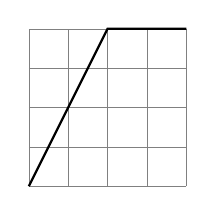
\begin{tikzpicture}
      \draw[step=0.5cm,gray,very thin] (0,0) grid (2,2);
      \draw[thick] (0,0) -- (1,2) -- (2,2);
    \end{tikzpicture}
    \quad
    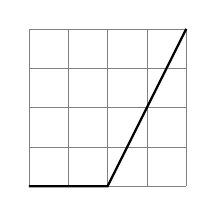
\begin{tikzpicture}
      \draw[step=0.5cm,gray,very thin] (0,0) grid (2,2);
      \draw[thick] (0,0) -- (1,0) -- (2,2);
    \end{tikzpicture}
    \quad
    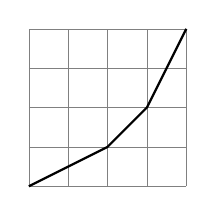
\begin{tikzpicture}
      \draw[step=0.5cm,gray,very thin] (0,0) grid (2,2);
      \draw[thick] (0,0) -- (1,0.5) -- (1.5,1) -- (2,2);
    \end{tikzpicture}
    \caption{Graphs of the functions $\phi_1$, $\phi_2$, and $\phi_3$ respectively.}
    \label{graph-reparametrisation}
  \end{figure}
  
  For (iii) we give a homotopy explicitly. Let us show that $\gamma \star \gamma^\inv \sim_p e_x$. For $t \in [0,1]$, define a path $\gamma_t : [0,1] \to X$ by $\gamma(s) = \gamma(ts)$, and define $G : [0,1] \times [0,1] \to X$ by
  \[
    G(s,t) = (\gamma_t \star \gamma_t^\inv)(s).
  \]
  That $G$ is continuous follows once again from an argument using Remark~\ref{pasting-closed}, and we see that $G$ is a homotopy from $e_x$ to $\gamma \star \gamma^\inv$ since
  \begin{align*}
    G(s,0) &= (\gamma_0 \star \gamma_0^\inv)(s) = \gamma(0) = x = e_x(s),\\
    G(s,1) &= (\gamma_1 \star \gamma_1^\inv)(s) = (\gamma \star \gamma^\inv)(s),\\
    G(0,t) &= \gamma_t(0) = \gamma(0) = x,\\
    G(1,t) &= \gamma_t^\inv(1) = \gamma(0) = x,
  \end{align*}
  for every $s$ and $t$. That $\gamma^\inv \star \gamma \sim_p e_y$ follows by an analogous argument.
\end{proof}


\subsection{The fundamental group}
The idea in this section will be to use the operation $\star$ on path homotopy classes to associate an algebraic structure to any pair $(X,x)$ for $X$ a topological space and $x \in X$. Moreover, when $X$ is path-connected, this structure will form a powerful topological invariant.

If $\gamma$ is a path from $x$ to $x$, we say that $\gamma$ is a \word{loop}{{\"o}gla} based at $x$.
\begin{defn}
  Let $X$ be a topological space, and let $x \in X$. Then the \word{fundamental group}{fundamentalgrupp} $\pi_1(X,x)$ is the set of all path homotopy classes of loops based at $x$. 
\end{defn}
\trans{fundamental group}{fundamentalgrupp}
To make sense of the terminology, let us recall a few basic notions from abstract algebra.
\begin{defn}
  A \word{group}{grupp} is a set $G$ with an operation $G \times G \to G$, denoted $(g,h) \mapsto g \cdot h$, an element $e \in G$ called a unit, and a bijection $G \to G$ denoted $x \mapsto x^{-1}$ called the inverse, so that
  \begin{itemize}
    \item $g \cdot (h \cdot k) = (g \cdot h) \cdot k$ for all $g,h,k \in G$,
    \item $e \cdot g = g = g \cdot e$ for all $g \in G$, and
    \item $g \cdot g^{-1} = g^{-1} \cdot g = e$ for all $g \in G$.
  \end{itemize}
  If $G$ and $H$ are groups, then a map $\phi : G \to H$ is called a \word{homomorphism}{homomorfi} if $\phi(g\cdot h) = \phi(g)\cdot\phi(h)$ for all $g,h \in G$. A bijective group homomorphism is called an \word{isomorphism}{isomorfi}.
\end{defn}
\trans{group}{grupp}
\trans{homomorphism}{homomorfi}
\trans{isomorphism}{isomorfi}
\begin{example}
  The one-point set $\{e\}$ is a group under the operation $(e,e) \mapsto e$. This group is called the \emph{trivial group}\index{trivial group}.
\end{example}
\begin{example}
  The integers form a group under the operation $(g,h) \mapsto g+h$. The unit is $0 \in \bbZ$, and if $n \in \bbZ$, then the inverse of $n$ is $-n$.
\end{example}
\begin{example}
  The set $\bbR \setminus \{0\}$ is a group with operation $(g,h) \mapsto gh$. The unit is $1$, and the inverse of $x \in \bbR \setminus \{0\}$ is $1/x$.
\end{example}
\begin{example}
  The set $\GL(n,\bbR)$ of invertible $(n \times n)$-matrices with entries in $\bbR$ is a group under matrix multiplication. The unit is the unit matrix.
\end{example}
\begin{prop}
  The fundamental group $\pi_1(X,x)$ is a group under the operation $\star$ on homotopy classes of loops for any topological space $X$ and any $x \in X$.
\end{prop}
\begin{proof}
  This follows immediately from Theorem~\ref{concatenation-homotopy}.
\end{proof} 

\begin{example}
  \label{fundemental-group-euclidean}
  In Example~\ref{euclidean-path-homotopy} we saw that any two given paths in $\bbR^n$ between the same points were homotopic. This in particular implies that any loop based at a point $x \in \bbR^n$ is null-homotopic; that is, homotopic to $e_x$. In other words,
  \[
    \pi_1(\bbR^n, x) = \{[e_x]\},
  \]
  the trivial group, for all $x \in \bbR^n$.
\end{example}
As the next thing, let us see how $\pi_1(X,x)$ depends on $x$.
\begin{thm}
  \label{fundamental-group-independent-of-basepoint}
  Let $X$ be a topological space, and let $\alpha$ be a path from $x$ to $y$ in $X$. Define a map $\hat{\alpha} : \pi_1(X,x) \to \pi_1(X,y)$ by
  \[
    \hat{\alpha}([\gamma]) = [\alpha^\inv] \star [\gamma] \star [\alpha].
  \]
  Then $\hat{\alpha}$ is well-defined and an isomorphism.
\end{thm}
\begin{proof}
  That $\hat{\alpha}$ is well-defined means that $\hat{\alpha}([\gamma]) = \hat{\alpha}([\gamma'])$ whenever $[\gamma] = [\gamma']$, i.e. whenever $\gamma \sim_p \gamma'$. And indeed, if $F: [0,1] \times [0,1] \to X$ is a path homotopy from $\gamma$ to $\gamma'$, then $G : [0,1] \times [0,1] \to X$, defined by
  \[
    G(s,t) = (\alpha^\inv \star F(\cdot,t) \star \alpha)(s)
  \]
  is a path homotopy from $\alpha^\inv \star \gamma \star \alpha$ to $\alpha^\inv \star \gamma' \star \alpha$, so $\hat{\alpha}$ is well-defined.

  To see that $\hat{\alpha}$ is an homomorphism, notice that for any $[\gamma], [\gamma'] \in \pi_1(X,x)$, we have
  \begin{align*}
    \hat{\alpha}([\gamma]) \star \hat{\alpha}([\gamma']) &= [\alpha^\inv] \star [\gamma] \star [\alpha] \star [\alpha^\inv] \star [\gamma'] \star [\alpha] \\
      &= [\alpha^\inv] \star ([\gamma] \star [\gamma']) \star [\alpha] = \hat{\alpha}([\gamma] \star [\gamma']).
  \end{align*}
  To see that $\hat{\alpha}$ is a bijection, notice that $\widehat{\alpha^\inv} \circ \hat{\alpha}$ is the identity on $\pi_1(X,x)$ since for any $[\gamma] \in \pi_1(X,x)$, we have
  \[
    (\widehat{\alpha^\inv} \circ \hat{\alpha})[\gamma] = \widehat{\alpha^\inv}([\alpha^\inv] \star [\gamma] \star [\alpha]) = [\alpha] \star [\alpha^\inv] \star [\gamma] \star [\alpha] \star [\alpha^\inv] = [\gamma],
  \]
  and $\hat{\alpha} \circ \widehat{\alpha^\inv}$ is the identity on $\pi_1(X,y)$ by the same reasoning, so $\hat{\alpha}$ is a bijection and thus a group isomorphism.
\end{proof}
\begin{cor}
  If $X$ is a path-connected topological space, then $\pi_1(X,x)$ is independent of $x \in X$ up to isomorphism.
\end{cor}
Because of this result, one often writes $\pi_1(X) = \pi_1(X,x)$ for any $x \in X$ when $X$ is path-connected. It is then understood that the equality is really up to isomorphism.
\begin{defn}
  A topological space $X$ is called \word{simply-connected}{enkelt sammanh{\"a}ngande} if it is path-connected and $\pi_1(X)$ consists of a single element.
\end{defn}
\begin{example}
  By Example~\ref{fundemental-group-euclidean}, $\bbR^n$ is simply-connected.
\end{example}

The next result says that for path-connected spaces, $\pi_1$ is a topological invariant. Even when the spaces in question are not path-connected, one obtains a topological invariant by considering the collection of groups $\pi_1(X,x_i)$ up to isomorphism, where each of the $x_i$ belongs to a different path-component of $X$.

As preparation, suppose that $f : X \to Y$ is a continuous map, and let $x \in X$. Define a map
\[
  f_* : \pi_1(X,x) \to \pi_1(Y,f(x))
\]
by
\[
  f_*([\gamma]) = [f \circ \gamma].
\]

\begin{thm}
  Let $f : X \to Y$ and $g : Y \to Z$ be continuous maps, and let $x \in X$. Then
  \begin{itemize}
    \item[(i)] $f_*: \pi_1(X,x) \to \pi_1(Y,f(x))$ is a well-defined homomorphism,
    \item[(ii)] $(g \circ f)_* = g_* \circ f_*$, and if $\id : X \to X$ denotes the identity, then $\id_* : \pi_1(X,x) \to \pi_1(X,x)$ is the identity on $\pi_1(X,x)$.
    \item[(iii)] Finally, if $f$ is a homeomorphism, then $f_*$ is an isomorphism.
  \end{itemize}
\end{thm}
\begin{proof}
  That $f_*$ is well-defined means that $f \circ \gamma \sim_p f \circ \gamma'$ whenever $\gamma \sim_p \gamma'$. This is the case since if $F$ is a homotopy from $\gamma$ to $\gamma'$, then $f \circ F$ is a homotopy from $f \circ \gamma$ to $f \circ \gamma'$.
  
  To see that $f_*$ is a homomorphism, let $[\gamma], [\gamma'] \in \pi_1(X,x)$ be arbitrary homotopy classes. We first notice that by definition of concatenation, we have
  \[
    f \circ ( \gamma \star \gamma') = (f \circ \gamma) \star (f \circ \gamma'),
  \]
  from which it follows that
  \begin{align*}
    f_*([\gamma] \star [\gamma']) &= f_*([\gamma \star \gamma']) = [f \circ (\gamma \star \gamma')] = [(f \circ \gamma) \star (f \circ \gamma')] \\
      &= [ f \circ \gamma] \star [f \circ \gamma'] = f_*([\gamma]) \star f_*([\gamma']),
  \end{align*}
  so $f_*$ is a homomorphism, which shows (i).
  
  Similarly,
  \[
    (g_* \circ f_*)([\gamma]) = g_* ( [f \circ \gamma]) = [g \circ f \circ \gamma] = (g \circ f)_*([\gamma]),
  \]
  which shows the first part of (ii). The last part of (ii) is obvious.
  
  Finally, (iii) follows from (ii) as it follows that $(f^{-1})_*$ satisfies that both $f_* \circ (f^{-1})_*$ and $(f^{-1})_* \circ f_*$ are the identity homomorphisms. Thus $f_*$ is a bijection and therefore an isomorphism.
\end{proof} 

If $G$ and $H$ are two groups, then their Cartesian product $G \times H$ is a group with the group operation
\[
  (g,h) \cdot (g',h') = (g\cdot g', h \cdot h').
\]
\begin{prop}
  \label{product-fundamental-group}
  Let $X$ and $Y$ be topological spaces, and let $x \in X$, $y \in Y$. Then $\pi_1(X \times Y,(x,y))$ is isomorphic to $\pi_1(X,x) \times \pi_1(Y,y)$.
\end{prop}
\begin{proof}
  Exercise~\ref{product-fundamental-group-exercise}.
\end{proof}

\subsection{Covering spaces and fundamental groups of spheres}
The main result of this section is a calculation of $\pi_1(S^n)$ for all $n \geq 1$.
\begin{thm}
  \label{fundamental-group-of-spheres}
  We have $\pi_1(S^1) = \bbZ$, but $S^n$ is simply-connected for $n \geq 2$.
\end{thm}

To prove the case $n = 1$, it will be convenient to have at our disposal some basic results about covering spaces. Before going into any detail about these, let us consider the ``easy'' part of the claim.
\begin{proof}[Proof of Theorem~\ref{fundamental-group-of-spheres} for $n \geq 2$]
  Let $\gamma$ be a loop in $S^n$, based at some point $\gamma(0)$, and let us show that $\gamma$ is null-homotopic. If there is a point $p$ not in the image of $\gamma$, we can view $\gamma$ as a loop in $S^n \setminus \{p\}$, which is homeomorphic to $\bbR^n$ by Remark~\ref{south-pole-removed}. Since $\bbR^n$ is simply-connected, this tells us that $\gamma$ is null-homotopic as a loop in $S^n \setminus \{ p \}$ through some homotopy $[0,1] \times [0,1] \to S^n \setminus \{p\}$. By composition with the inclusion, this gives us a homotopy $[0,1] \times [0,1] \to S^n$, so $\gamma$ is also null-homotopic as a loop in $S^n$.
  
  This shows the claim in the case where $\gamma([0,1]) \not= S^n$. Now, let $p$ be a point in $S^n$ distinct from $\gamma(0)$. We will show how to make a path homotopy from $\gamma$ to some other loop, denoted $\gamma_k$ below, whose image does not contain $p$. This other loop will then be null-homotopic by the first part of the proof, so $\gamma$ will be as well.
  
  Let $U$ be any neighbourhood of $p$ which does not contain $\gamma(0)$. After possibly having to pass to a smaller neighbourhood we can assume that $U$ is homeomorphic to an open ball in $\bbR^n$. Now $\gamma^{-1}(U) \subset (0,1) \subset [0,1]$ is an open set and therefore a union of open disjoint intervals $(a_i,b_i)$, $i \in I$. Since $\{p\}$ is closed in $S^n$, $\gamma^{-1}(\{p\})$ is closed in $[0,1]$, and since $[0,1]$ is compact, so is $\gamma^{-1}(\{p\})$. Since $\{(a_i,b_i)\}_{i \in I}$ is an open cover of $\gamma^{-1}(\{p\})$, this compactness implies that we can find finitely many intervals $(a_1,b_1), \dots, (a_k,b_k)$ that cover $\gamma^{-1}(\{p\})$. We will now cook up the desired homotopy for each of these finitely many intervals.
  
  Since $(a_1,b_1) \subset \gamma^{-1}(U)$ with $a_1,b_1 \notin \gamma^{-1}(U)$, we get that $\gamma([a_1,b_1]) \subset \bar{U}$ and $\gamma(a_1),\gamma(b_1) \in \dd U$. Now take any path $\widetilde{\gamma_1}$ in $\bar{U}$ from $\gamma(a_1)$ to $\gamma(b_1)$ which does not go through $p$. Since $U$ was assumed to be homeomorphic to a ball, $\gamma|_{[a_1,b_1]}$ is path homotopic to $\widetilde{\gamma_1}$ (ignoring the minor detail that the paths in question have to be defined on $[0,1]$) and this path homotopy extends to a path homotopy from $\gamma$ to some loop $\gamma_1$ with the property that $p \notin \gamma_1([a_1,b_1])$ and so that $\gamma_1$ agrees with $\gamma$ on the complement of $[a_1,b_1]$ in $[0,1]$. We now iterate this procedure to obtain for each $j = 1, \dots, k$ a loop $\gamma_j$ so that $\gamma \sim_p \gamma_j$ and $p \notin \gamma_j([a_1,b_1] \cup \dots \cup [a_j,b_j])$. Then $p \notin \gamma_k([0,1])$ and $\gamma \sim \gamma_k$, so we are done.
\end{proof}

Before moving on to the case $n = 1$, let us notice the following non-trivial corollary of the theorem.
\begin{cor}
  We have $S^n \simeq T^m$ if and only if $n = m = 1$.
\end{cor}
\begin{proof}
  By Proposition~\ref{product-fundamental-group} and Theorem~\ref{fundamental-group-of-spheres}, $\pi_1(T^m) = \pi_1(S^1 \times \cdots \times S^1)$ is the product of $m$ copies of $\bbZ$. Since $\bbZ^m$ is not isomorphic to $\bbZ$ if $m > 1$, $\pi_1(T^m)$ can only be isomorphic to $\pi_1(S^n)$ if $n = m = 1$.
\end{proof}
\begin{wrapfigure}{R}{0.3\textwidth}
  \centering
  \begin{overpic}[width=0.28\textwidth]{images/covering}
    \put(37,60){$E$}
    \put(37,13){$B$}
    \put(24,33){$p$}
    \put(18,17){$U$}
    \put(13,91){$p^{-1}(U)$}
  \end{overpic}
  \caption{A covering map $p : E \to B$.}
  \label{covering-figure}
\end{wrapfigure}
% \trans{covering space}{?}
% \trans{covering map}{?}
\begin{defn}
  Let $B$ be a topological space. A \wordnotrans{covering space}{?} of $B$ is a topological space $E$ and a continuous surjective map $p : E \to B$, called a \wordnotrans{covering map}{?}, so that each point $b \in B$ has an open neighbourhood $U$ with the property that $p^{-1}(U)$ is a disjoint union of open sets in $E$, each of which is mapped homeomorphically to $U$ by $p$. See Figure~\ref{covering-figure}.
\end{defn}

\begin{example}
  \label{covering-of-circle}
  The real line $\bbR$ is a covering space of $S^1$ with covering map $p : \bbR \to S^1$ given by $p(x) = (\cos(2\pi x), \sin(2\pi x))$.
\end{example}

\begin{defn}
  Let $p : E \to B$ be a covering map, and let $f : X \to B$ be a continuous map. A map $\tilde{f} : X \to E$ is called a \word{lifting}{l{\"o}ft} of $f$ if $f = p \circ \tilde{f}$.
\end{defn}
\trans{lifting}{l{\"o}ft}

The two following lemmas will be proven in Section~\ref{proofs-lifting-lemmas} below.
\begin{lem}[Path lifting lemma]
  \label{path-lifting-lemma}
  \index{path lifting lemma}Let $p : E \to B$ be a covering map, let $b \in B$, and let $e \in E$ with $p(e) = b$. Then any path $\gamma : [0,1] \to B$ with $\gamma(0) = b$ has a unique lifting $\tilde{\gamma} : [0,1] \to E$ so that $\tilde{\gamma}(0) = e$.
\end{lem}

\begin{lem}[Homotopy lifting lemma]
  \label{homotopy-lifting-lemma}
  \index{homotopy lifting lemma}Let $p : E \to B$ be a covering map, and let $p(e) = b$ as above. Let $F : [0,1] \times [0,1] \to B$ be a homotopy with $F(0,0) = b$. Then there is a a unique lifting $\tilde{F} : [0,1] \times [0,1] \to E$ so that $\tilde{F}(0,0) = e$. If $F$ is a path homotopy then so is $\tilde{F}$.
\end{lem}

Now as above, let $p : E \to B$ be a covering map, let $b \in B$, and choose $e \in E$ with $p(e) = b$. Let $[\gamma] \in \pi_1(B,b)$ be a homotopy class of a path $\gamma$, and let $\tilde{\gamma}$ be the unique lifting from Lemma~\ref{path-lifting-lemma}, with $\tilde{\gamma}(0) = e$. Define a map, called the \word{lifting correspondence}{?},
\[
  \phi_e : \pi_1(B,b) \to p^{-1}(\{b\})
\]
by $\phi_e([\gamma]) = \tilde{\gamma}(1)$. To see that this is well-defined, assume that $\gamma \sim_p \gamma'$, and let $F$ denote a path homotopy from $\gamma$ to $\gamma'$. Then the unique lifting $\tilde{F}$ from Lemma~\ref{homotopy-lifting-lemma} is a path homotopy from $\tilde{\gamma}$ to $\widetilde{\gamma'}$, and in particular $\tilde{\gamma}(1) = \widetilde{\gamma'}(1)$.

\begin{prop}
  \label{lifting-correspondence-props}
  Let $p : E \to B$, $p(e) = b$, be as above. If $E$ is path-connected then $\phi_e$ is surjective. If $E$ is simply-connected, then $\phi_e$ is bijective.
\end{prop}
\begin{proof}
  Assume first that $E$ is path-connected and let $q \in p^{-1}(\{b\})$. Choose any path $\tilde{\gamma}$ from $e$ to $q$, and let $\gamma = p \circ \tilde{\gamma}$. Then $\tilde{\gamma}$ is a lift of $\gamma$ by construction, and $\phi_e([\gamma]) = q$, so $\phi_e$ is surjective.
  
  Assume now that $E$ is simply-connected, suppose that $\phi_e([\gamma]) = \phi_e([\gamma'])$ for two elements $[\gamma], [\gamma'] \in \pi_1(B,b)$, and let us show that $[\gamma] = [\gamma']$. Let $\tilde{\gamma}$ and $\widetilde{\gamma'}$ denote the corresponding lifts, so that $\tilde{\gamma}(1) = \tilde{\gamma'}(1)$ by assumption. Then $\tilde{\gamma} \star \widetilde{\gamma'}^\inv$ is a loop based at $e$ and thus path homotopic to the constant map since $E$ is simply-connected. This implies that
  \[
    [\tilde{\gamma}] = [\tilde{\gamma}] \star [\widetilde{\gamma'}^\inv] \star [\widetilde{\gamma'}] = [\tilde{\gamma} \star \widetilde{\gamma'}^\inv] \star [\widetilde{\gamma'}] = [\widetilde{\gamma'}],
  \]
  so there is a path homotopy $\tilde{F}$ from $\tilde{\gamma}$ to $\widetilde{\gamma'}$. Then $p \circ \tilde{F}$ is a path homotopy from $p \circ \tilde{\gamma} = \gamma$ to $p \circ \widetilde{\gamma'} = \gamma'$, or in other words, $[\gamma] = [\gamma']$.
\end{proof}

We are now in a position to prove our main result.
\begin{proof}[Proof of Theorem~\ref{fundamental-group-of-spheres} for $n = 1$]
  Let $p : \bbR \to S^1$ be the covering map from Example~\ref{covering-of-circle}, let $b = (1,0) \in S^1$, and let $e = 0$. In this case, since $p^{-1}(\{b\}) = \bbZ$, and since $\bbR$ is simply-connected, Proposition~\ref{lifting-correspondence-props} implies that $\phi_e : \pi_1(S^1,b) \to \bbZ$ is bijective, and we claim that it is a homomorphism.
  
  Let $m \in \bbZ$, and let $\gamma_m : [0,1] \to \bbZ$ be the loop given by
  \[
    \gamma_m(t) = (\cos(2\pi mt), \sin(2\pi mt)).
  \]
  This loop lifts to $\widetilde{\gamma_m} : [0,1] \to \bbR$ given by $\widetilde{\gamma_m}(t) = mt$. This tells us that $\phi_e([\gamma_m]) = m$. Since $\phi_e$ was a projection, each loop $\gamma$ based at $b$ will belong to $[\gamma_m]$ for some $m \in \bbZ$, so to show that $\phi_e$ is a homomorphism, it suffices to show that
  \[
    \phi_e([\gamma_m \star \gamma_n]) = m + n = \phi_e([\gamma_m]) + \phi_e([\gamma_n]),
  \]
  for all $m , n \in \bbZ$. Let $\widetilde{\gamma_n^m} = m + \widetilde{\gamma_n}$ be the lifting of $\gamma_n$ starting at $m$ and ending at $m+n$. Then $\widetilde{\gamma_m} \star \widetilde{\gamma_n^m}$ is a path from $0$ to $m+n$ and $p \circ (\widetilde{\gamma_m} \star \widetilde{\gamma_n^m}) = \gamma_m \star \gamma_n$, so by definition of $\phi_e$, this tells us that $\phi_e([\gamma_m \star \gamma_n]) = m+n$.
\end{proof}

Up until this point, it is not clear how useful $\pi_1$ actually is as an invariant: indeed, most of the calculations of fundamental groups that we have done turned out to yield trivial groups, and, for instance, we can not use the fundamental group to tell apart the spaces $\bbR^n$ and $S^n$ for $n \geq 2$, even though one can show by elementary means that these spaces are non-homeomorphic.

Restricting to the class of manifolds considered in Section~\ref{manifolds} one can say quite a bit more. It is not too difficult to prove, for instance, that if a $2$-manifold is compact and simply-connected, then it is homeomorphic to $S^2$. That is, the fundamental group can detect $S^2$ among all compact $2$-manifolds. The same statement holds true for $3$-manifolds, although it is currently significantly harder to prove.
\begin{thm}[The Poincar{\'e} conjecture]
  \index{Poincar{\'e} conjecture}If $X$ is a simply-connected compact $3$-manifold, then $X \simeq S^3$.
\end{thm}
Conjectured by Henri Poincar{\'e} in 1904, and first proven by Grigori Perelman in 2003, at the time of writing this is the only solved out of the seven so-called Millennium Prize Problems\footnote{See \url{https://en.wikipedia.org/wiki/Millennium_Prize_Problems}.}.

\subsection{Proofs of lifting lemmas}
\label{proofs-lifting-lemmas}
We now turn to the proofs of Lemmas~\ref{path-lifting-lemma} and \ref{homotopy-lifting-lemma} where we will need a technical result on subdivisions of $[0,1]$ and $[0,1] \times [0,1]$. We word it here for general compact metric spaces.

Let $(X,d)$ be a metric space, and let $A$ be a non-empty subset. Then for every $x \in X$, we define the distance from $x$ to $A$ by
\[
  d(x,A) = \inf \{ d(x,a) \mid a \in A \}.
\]
It is easy to see that for fixed $A$, the function $x \mapsto d(x,A)$ is continuous. If moreover $A$ is bounded in the sense that the set $\{d(a_1,a_2) \mid a_1,a_2 \in A\} \subset \bbR$ is bounded, we define the \word{diameter}{diameter} of $A$ to be
\[
  \diam(A) = \sup \{d(a_1,a_2) \mid a_1,a_2 \in A \} \in \bbR.
\]
\begin{lem}[Lebesgue's number lemma]
  \label{lebesgue-number-lemma}
  \index{Lebesgue's number lemma}Let $\calU$ be an open cover of a compact metric space $(X,d)$. Then there is a $\delta > 0$, called a \index{Lebesgue number}\emph{Lebesgue number}, so that for every subset $A$ of diameter less than $\delta$, there is a $U \in \calU$ with $A \subset U$.
\end{lem}
\begin{proof}
  First of all, if $X \in \calU$, we are done since any $\delta > 0$ does the job, so assume that $X \notin \calU$.

  Now use the compactness of $X$ to take an finite subcover $\{U_1,\dots,U_n\} \subset \calU$. Let $C_i = X \setminus U_i \not= \emptyset$ for $i = 1, \dots, n$, and define a function $f : X \to \bbR$ by
  \[
    f(x) = \frac{1}{n} \sum_{i=1}^n d(x,C_i).
  \]
  We claim that $f(x) > 0$ for all $x \in X$. To see this, let $x \in X$ and choose an $i$ so that $x \in U_i$. Since $U_i$ is open, we can find a $\eps > 0$ so that $B(x,\eps) \subset U_i$. Then $d(x,C_i) \geq \eps$, so $f(x) \geq \eps/n > 0$. Since $f$ is continuous, it follows from Corollary~\ref{sup-inf-compact-continuous} that $f(X)$ has a minimum $\delta > 0$, and we now claim that this number is our desired Lebesgue number.
  
  Let $A \subset X$ have diameter less than $\delta$, and let $a \in A$. Then $A \subset B_d(a,\delta)$, and by taking $m \in \{1,\dots,n\}$ so that $d(a,C_m)$ is maximal, we have
  \[
    \delta \leq f(a) \leq d(a,C_m),
  \]
  so $A \subset B_d(a,\delta) \subset X \setminus C_m = U_m$.
\end{proof}
We can now prove the two lemmas.% As will be clear, the two proofs are very similar, and indeed one could view both of them as following from a more general result on liftings of homotopies. To simplify the exposition, however, we prove the claims separately.
\begin{proof}[Proof of Lemma~\ref{path-lifting-lemma}]
  Choose an open cover $\calU$ of $B$ by sets $U \in \calU$ with the property that $p^{-1}(U)$ is a disjoint union of open sets in $E$, each of which is mapped homeomorphically to $U$ by $p$.
  
  Now $\{\gamma^{-1}(U) \mid U \in \calU\}$ is an open cover of the compact set $[0,1]$. By Lemma~\ref{lebesgue-number-lemma}, there is a subdivision $0 = s_0 < s_1 < \dots < s_n = 1$ of $[0,1]$ so that for every $i = 1, \dots, k$, we have $[s_{i-1},s_i] \subset \gamma^{-1}(U)$ for some $U \in \calU$. That is, $\gamma([s_{i-1},s_i]) \subset U$. We will now construct the lifting $\tilde{\gamma}$ on each of these smaller intervals through a finite induction.
  
  Let $\tilde{\gamma}(0) = e$ and assume that the lifting $\tilde{\gamma}$ has been defined on $[0,s_i]$. We then define $\tilde{\gamma}$ on $[s_i,s_{i+1}]$ as follows: let $V \in \calU$ be the open set so that $\gamma([s_i,s_{i+1}]) \subset U$. Then $\tilde{\gamma}(s_i) \in p^{-1}(U)$, so we can choose $V \subset E$ so that $p|_V : V \to U$ is a homeomorphism and $\tilde{\gamma}(s_i) \in V$. Now, for any $s \in [s_i,s_{i+1}]$, we can define
  \[
    \tilde{\gamma}(s) = (p|_V)^{-1}(\gamma(s)).
  \]
  Then $\tilde{\gamma}$ is continuous on $[s_i,s_{i+1}]$, agrees with $\tilde{\gamma}$ on the set $\{s_i\}$, and so defines a function $\tilde{\gamma} : [0,s_{i+1}] \to E$ which is continuous by the pasting lemma, Remark~\ref{pasting-closed}. Moreover, $\tilde{\gamma}$ is constructed to satisfy $\gamma = p \circ \tilde{\gamma}$ where it is defined, so repeating this procedure $n$ times we obtain our desired lift.
  
  It remains to prove that $\tilde{\gamma}$ is unique. Suppose that $\tilde{\gamma}'$ is another lifting of $\gamma$ with $\tilde{\gamma}'(0) = e$, and suppose that $\tilde{\gamma} = \tilde{\gamma}'$ on $[0,s_i]$ (which we know is true for $i=0$). We then claim that the lifts agree on $[0,s_{i+1}]$ as well, and therefore $\tilde{\gamma} = \tilde{\gamma}'$ on all of $[0,1]$, so let $s \in [s_i,s_{i+1}]$, and let $V$ be as above so that $\tilde{\gamma}(s_i), \tilde{\gamma}'(s_i) \in V$.
  
  Since $[s_i,s_{i+1}]$ is connected, so is the set $\tilde{\gamma}'([s_i,s_{i+1}])$ by Theorem~\ref{images-of-connected}, and therefore it must be contained in a single connected component by Proposition~\ref{props-of-conn-components}. Now, since the open sets making up $p^{-1}(U)$ are disjoint, this implies that $\tilde{\gamma}'([s_i,s_{i+1}]) \subset V$, so in particular $\tilde{\gamma}'(s) \in V$. Now, since $p|_V : V \to U$ is bijective, there is only one point in $V$ that is mapped to $\gamma(s)$ under $p$, namely $(p|_V)^{-1}(\gamma(s))$, so since $\tilde{\gamma}'$ is a lifting of $\gamma$, it follows that
  \[
    \tilde{\gamma}'(s) = (p|_V)^{-1}(\gamma(s)) = \tilde{\gamma}(s).
  \]
\end{proof}

\begin{proof}[Proof of Lemma~\ref{homotopy-lifting-lemma}]
  \begin{figure}
    \centering
    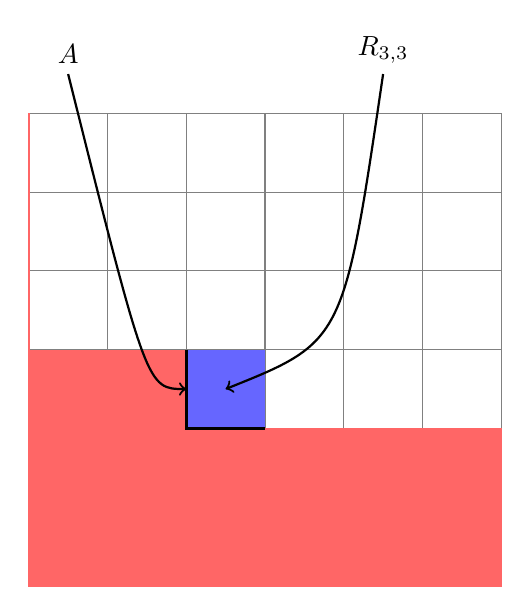
\begin{tikzpicture}
      \draw[step=1cm,gray] (0,0) grid (6,6);
      \fill[red!60!white] (0,0) rectangle (2,3);
      \fill[red!60!white] (0,0) rectangle (6,2);
      \fill[blue!60!white] (2,2) rectangle (3,3);
      \draw[red!60!white,thick] (0,6) -- (0,0) -- (6,0) -- (6,2);% -- (3,2);
      %\draw[red!60!white,thick] (0,3) -- (2,3);
      %\draw[blue!60!white,thick] (3,2) -- (3,3) -- (2,3);
      \draw[very thick] (2,3) -- (2,2) -- (3,2);
      \draw[thick,<-] (2.5,2.5) .. controls (4,3.1) .. (4.5,6.5) node[anchor=south]{$R_{3,3}$};
      \draw[thick,<-] (2,2.5) .. controls (1.5,2.5) .. (0.5,6.5) node[anchor=south]{$A$};
    \end{tikzpicture}
    \caption{The sets involved in the proof of Lemma~\ref{homotopy-lifting-lemma}. The red part indicates where $\tilde{F}$ has been defined, and the blue part where we are in the process of defining $\tilde{F}$.}
    \label{homotopy-lifting-figure}
  \end{figure}
  As in the proof above, we will define a lift $\tilde{F}$ in a step-by-step fashion, so let $\calU$ denote an open cover $B$ as above. Begin by letting $\tilde{F}(0,0) = e$, and use Lemma~\ref{path-lifting-lemma} to uniquely define $\tilde{F}$ on $[0,1] \times \{0\}$ and $\{0\} \times [0,1]$, lifting $F$ on these subsets.
  
  As above, we can now consider $\{F^{-1}(U) \mid U \in \calU\}$ and conclude by Lemma~\ref{lebesgue-number-lemma} that there exist subdivisions $0 = s_0 < s_1 < \dots < s_m = 1$ and $0 = t_0 < t_1 < \dots < t_n = 1$ so that for each rectangle
  \[
    R_{i,j} = [s_{i-1},s_i] \times [t_{j-1},t_j] \subset [0,1] \times [0,1]
  \]
  there is a $U \in \calU$ with $F(R_{i,j}) \subset U$. We now define $\tilde{F}$ on the rectangles $R_{i,j}$ in the order
  \[
    R_{1,1}, R_{2,1}, \dots, R_{m,1}, R_{1,2}, R_{2,2}, \dots, R_{m,2}, \dots, R_{1,n}, R_{2,n}, \dots, R_{m,n}.
  \]
  Assume that the lifting $\tilde{F}$ has been defined on all rectangles up to a certain point, and let us define $\tilde{F}$ on the next rectangle $R_{i,j}$. In particular, $\tilde{F}$ has been defined on $A$: the union of the left and bottom edge of $R_{i,j}$, which is a connected set (see Figure~\ref{homotopy-lifting-figure}). By the exact same logic as in the previous proof, this implies $\tilde{F}(A) \subset V$, where $V \subset E$ is so that $p|_V : V \to U$ is a homeomorphism and $F(R_{i,j}) \subset U$. This means that we can extend $\tilde{F}$ to $R_{i,j}$ by letting
  \[
    \tilde{F}(x) = (p|_V)^{-1}(F(x)).
  \]
  Proceeding like this for all rectangles, we define $\tilde{F}$ on all of $[0,1] \times [0,1]$. Then $\tilde{F}$ is continuous by the pasting lemma and a lifting of $F$ by construction. That $\tilde{F}$ is the unique lifting with $\tilde{F}(0,0) = e$ follows by the same logic as in the proof of Lemma~\ref{path-lifting-lemma} above.
  
  It remains to show that if $F$ is a path homotopy, then so is $\tilde{F}$. So, assume that $F([0,1] \times \{0\}) = \{b\}$. Then $\tilde{F}([0,1]\times\{0\}) \subset p^{-1}(\{b\})$. Now $[0,1] \times \{0\}$ is connected, so its image under $\tilde{F}$ is connected, and on the other hand, $p^{-1}(\{b\})$ is discrete so its connected components are points, which means that $\tilde{F}$ is constant on $[0,1] \times \{0\}$. Similarly, if $F$ is constant on $[0,1] \times \{1\}$, one uses connectedness to argue that $\tilde{F}$ is as well.
\end{proof}
